\documentclass[xcolor=dvipsnames,11pt]{beamer}

\usepackage{amssymb,amsfonts}
\usepackage{amsmath}
\usepackage{booktabs}
\usepackage{lmodern}
\usepackage{graphicx}
\usepackage{tikz}
\usepackage{verbatim}

\usefonttheme[onlymath]{serif}
\setbeamerfont{frametitle}{size=\large, shape=\normalfont}
\vfuzz=25pt
\hbadness=10000
\vbadness=10000

\usetheme{Copenhagen}
\usecolortheme[RGB={240,160,40}]{structure}
\setbeamertemplate{navigation symbols}{}
\setbeamertemplate{footline}[frame number]


\title{The Hardness of $H$-Free Edge Editing}
\author{{\bf N.R.Aravind} }
\institute{Indian Institute of Technology Hyderabad}
\date{}

\begin{document}

\maketitle

\frame
{
\frametitle{$H$-Free Graphs}

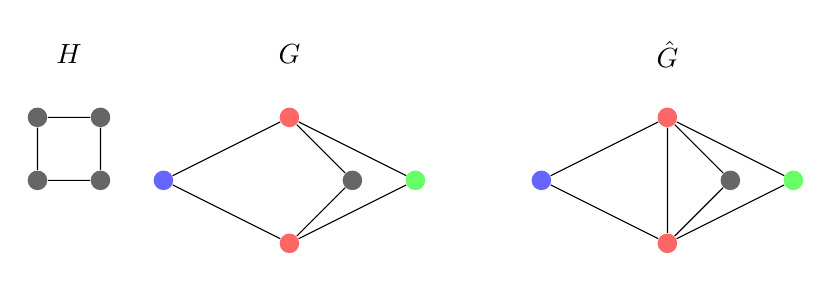
\begin{tikzpicture}
	 [scale=.8,auto=center,every node/.style={circle,fill=black!60,inner sep=2.5pt}]
	\node[fill=none] at (6.5,9) {$H$};
	\node[fill=none] at (10,9) {$G$};

	  \node (a)[fill=red!60] at (10,8) {};
	  \node (b)[fill=red!60] at (10,6) {};
	  \node (c)[fill=blue!60] at (8,7) {};
 	  \node (d) at (11,7) {};
	  \node (e)[fill=green!60] at (12,7) {};


	\foreach \from/\to in {a/c,a/d,a/e,b/c,b/d,b/e}
    \draw (\from) -- (\to);

    \node (p) at (6,7) {};
    \node (q) at (7,7) {};
    \node (r) at (7,8) {};
    \node (s) at (6,8) {};
    \foreach \from/\to in {p/q,q/r,r/s,s/p}
    \draw (\from) -- (\to);

	\node[fill=none] at (16,9) {$\hat{G}$};
	  \node (a1)[fill=red!60] at (16,8) {};
	  \node (b1)[fill=red!60] at (16,6) {};
	  \node (c1)[fill=blue!60] at (14,7) {};
 	  \node (d1) at (17,7) {};
	  \node (e1)[fill=green!60] at (18,7) {};


	\foreach \from/\to in {a1/c1,a1/d1,a1/e1,b1/c1,b1/d1,b1/e1,a1/b1}
    \draw (\from) -- (\to);

\end{tikzpicture}

\vspace{2mm}
$G$ is $C_4$-free, i.e. has no induced copies of $C_4$.
}


\frame
{
\frametitle{HEE}

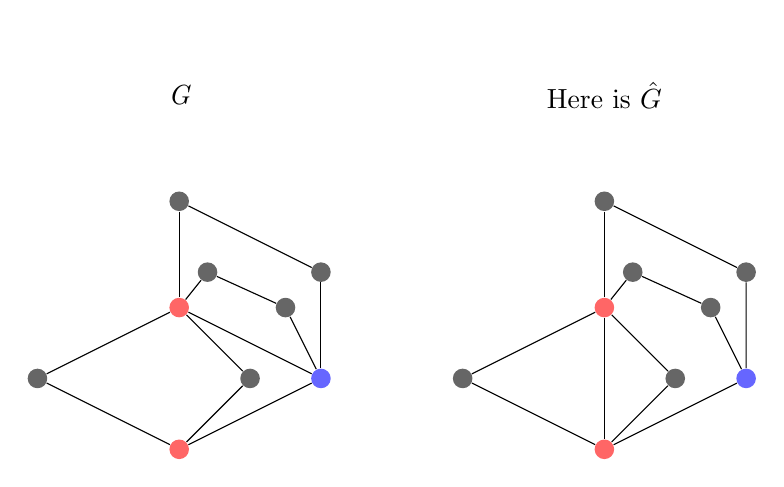
\begin{tikzpicture}
	 [scale=.9,auto=center,every node/.style={circle,fill=black!60,inner sep=2.5pt}]
	\node[fill=none] at (6,11) {$\textit{G}$}       ;

	  \node (a)[fill=red!60] at (6,8) {};
	  \node (b)[fill=red!60] at (6,6) {};
	  \node (c) at (4,7) {};
 	  \node (d) at (7,7) {};
	  \node (e) at (8,7)[fill=blue!60] {};

	\node(p) at (6.4,8.5) {};
	\node(q) at (7.5,8) {};

	\node(r) at (6,9.5) {};
	\node(s) at (8,8.5) {};

	\foreach \from/\to in {a/c,a/d,a/e,b/c,b/d,b/e,a/p,e/q,a/r,e/s,p/q,r/s}
    \draw (\from) -- (\to);


	\node[fill=none] at (12,11) {Here is $\hat{G}$};

	 \node (a1)[fill=red!60] at (12,8) {};
	  \node (b1)[fill=red!60] at (12,6) {};
	  \node (c1) at (10,7) {};
 	  \node (d1) at (13,7) {};
	  \node (e1) at (14,7)[fill=blue!60] {};

	\node(p1) at (12.4,8.5) {};
	\node(q1) at (13.5,8) {};

	\node(r1) at (12,9.5) {};
	\node(s1) at (14,8.5) {};

	\foreach \from/\to in {a1/c1,a1/d1,a1/b1,b1/c1,b1/d1,b1/e1,a1/p1,e1/q1,a1/r1,e1/s1,p1/q1,r1/s1}
    \draw (\from) -- (\to);

\end{tikzpicture}
}


\frame
{
\frametitle{Reduction from high-degree vertices}

\begin{lemma} \label{lem:degree}
$H$-FEE $\succcurlyeq$ $H_1$-FEE, where
$H_1=H[v: deg(v)>d]$.
\end{lemma}

\vspace{1mm}

\begin{center}
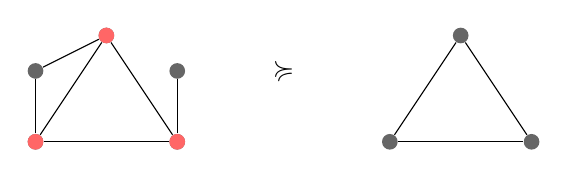
\begin{tikzpicture}
	 [scale=.9,auto=center,every node/.style={circle,fill=black!60,inner sep=2pt}]
%	\node[fill=none] at (13,9) {$H$};

	  \node (a) at (13,7.5) {};
	  \node (b) at (12,6) {};
	  \node (c) at (14,6) {};
	  \node (d) at (12,7) {};
 	  \node (e) at (14,7) {};

	\foreach \from/\to in {a/b,b/c,c/a,a/d,b/d,c/e}
    \draw (\from) -- (\to);

	 \node (a1)[fill=red!60] at (13,7.5) {};
	  \node (b1)[fill=red!60] at (12,6) {};
	  \node (c1)[fill=red!60] at (14,6) {};

    \node[fill=none] at (15.5,7) {$\succcurlyeq$};

%	\node[fill=none] at (18,9) {$H_1$};

	  \node (r) at (18,7.5) {};
	  \node (s) at (17,6) {};
 	  \node (t) at (19,6) {};

\foreach \from/\to in {r/s,s/t,t/r}
    \draw (\from) -- (\to);

\end{tikzpicture}
\end{center}
}


\frame
{
\frametitle{High-degree reduction}

\begin{center}
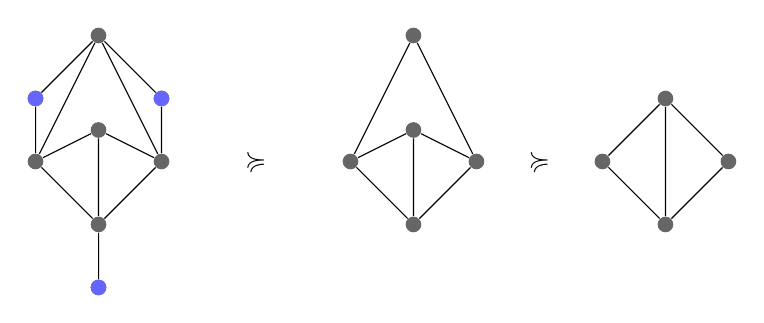
\begin{tikzpicture}
	 [scale=.8,auto=center,every node/.style={circle,fill=black!60,inner sep=2pt}]

	  \node (n1) at (12,6) {};
	  \node (n2) at (12,7) {};
	  \node (n3) at (13,8) {};
	  \node (n4) at (14,7) {};
 	  \node (n5) at (14,6) {};
	  \node (n6) at (13,5) {};
   	  \node (n7) at (13,4) {};
	  \node (n8) at (13,6.5) {};
	\foreach \from/\to in {n1/n2,n2/n3,n3/n4,n4/n5,n5/n6,n6/n7,n1/n6,n6/n8,n1/n8,n5/n8,n1/n3,n5/n3}
    \draw (\from) -- (\to);

	  \node (n12) [fill=blue!60] at (12,7) {};
	  \node (n14) [fill=blue!60] at (14,7) {};
   	  \node (n17) [fill=blue!60] at (13,4) {};

   \node[fill=none] at (15.5,6) {$\succcurlyeq$};

	  \node (m1) at (17,6) {};
	  \node (m3) at (18,8) {};
 	  \node (m5) at (19,6) {};
	  \node (m6) at (18,5) {};
  	  \node (m8) at (18,6.5) {};

	\foreach \from/\to in {m1/m6,m5/m6,m6/m8,m1/m8,m5/m8,m1/m3,m5/m3}
    \draw (\from) -- (\to);

 \node[fill=none] at (20,6) {$\succcurlyeq$};

	  \node (a) at (21,6) {};
 	  \node (b) at (23,6) {};
	  \node (c) at (22,5) {};
  	  \node (d) at (22,7) {};

	\foreach \from/\to in {a/c,b/c,c/d,a/d,b/d}
    \draw (\from) -- (\to);


\end{tikzpicture}
\end{center}
}


\frame{
\frametitle{Obstacle 1: Regular graphs}

\begin{center}
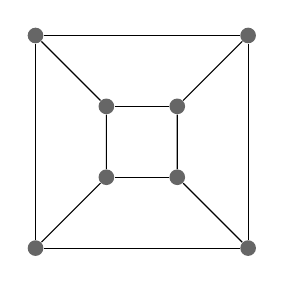
\begin{tikzpicture}
	 [scale=.9,auto=center,every node/.style={circle,fill=black!60,inner sep=2pt}]

  \node (a) at (17,6) {};
    \node (b) at (18,6) {};
    \node (c) at (18,7) {};
    \node (d) at (17,7) {};
    \foreach \from/\to in {a/b,b/c,c/d,d/a}
    \draw (\from) -- (\to);

	 \node (x) at (16,5) {};
    \node (y) at (19,5) {};
    \node (z) at (19,8) {};
    \node (t) at (16,8) {};
    \foreach \from/\to in {x/y,y/z,z/t,t/x,a/x,b/y,c/z,d/t}
    \draw (\from) -- (\to);

\end{tikzpicture}
\end{center}
}


\frame
{
\frametitle{Obstacle 2: Easy graphs}

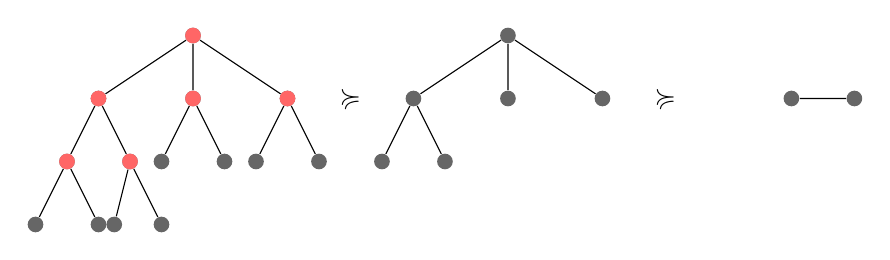
\begin{tikzpicture}
	 [scale=.8,auto=center,every node/.style={circle,fill=black!60,inner sep=2pt}]

	  \node (m1) at (11.5,5) {};
	  \node (m2) at (10,4) {};
	  \node (m3) at (11.5,4) {};
	  \node (m4) at (13,4) {};
 	  \node (m5) at (9.5,3) {};
	  \node (m6) at (10.5,3) {};
   	  \node (m7) at (11,3) {};
	  \node (m8) at (12,3) {};
	  \node (m9) at (12.5,3) {};
 	  \node (m0) at (13.5,3) {};
	  \node (r) at (9,2) {};
   	  \node (s) at (10,2) {};
	  \node (t) at (10.25,2) {};
   	  \node (u) at (11,2) {};

	\foreach \from/\to in {m1/m2,m1/m3,m1/m4,m2/m5,m2/m6,m3/m7,m3/m8,m4/m9,m4/m0,m5/r,m5/s,m6/t,m6/u}
    \draw (\from) -- (\to);

	 \node (m11)[fill=red!60] at (11.5,5) {};
	  \node (m21)[fill=red!60] at (10,4) {};
	  \node (m31)[fill=red!60] at (11.5,4) {};
	  \node (m41)[fill=red!60] at (13,4) {};
 	  \node (m51)[fill=red!60] at (9.5,3) {};
	  \node (m61)[fill=red!60] at (10.5,3) {};

   	\node[fill=none] (L2) at (14,4) {$\succcurlyeq$};
        \node (x1) at (16.5,5) {};
	  \node (x2) at (15,4) {};
	  \node (x3) at (16.5,4) {};
	  \node (x4) at (18,4) {};
 	  \node (x5) at (14.5,3) {};
	  \node (x6) at (15.5,3) {};

	\foreach \from/\to in {x1/x2,x1/x3,x1/x4,x2/x5,x2/x6}
    \draw (\from) -- (\to);

	\node[fill=none] (L3) at (19,4) {$\succcurlyeq$};

    	  \node (b1) at (21,4) {};
	  \node (b2) at (22,4) {};

	\foreach \from/\to in {b1/b2}
    \draw (\from) -- (\to);

\end{tikzpicture}
}



\frame
{
\frametitle{Easy graphs: Using Complement Equivalence}

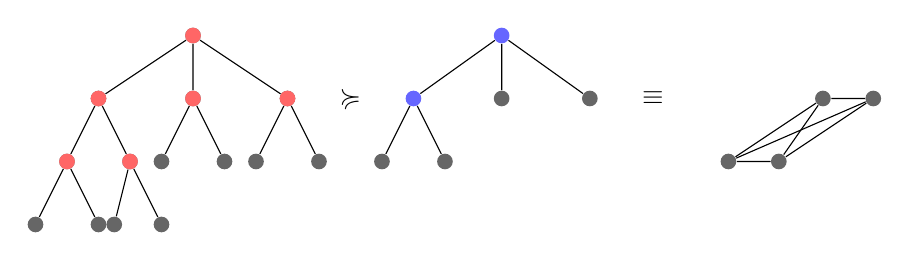
\begin{tikzpicture}
	 [scale=.8,auto=center,every node/.style={circle,fill=black!60,inner sep=2pt}]

	  \node (m1) at (11.5,5) {};
	  \node (m2) at (10,4) {};
	  \node (m3) at (11.5,4) {};
	  \node (m4) at (13,4) {};
 	  \node (m5) at (9.5,3) {};
	  \node (m6) at (10.5,3) {};
   	  \node (m7) at (11,3) {};
	  \node (m8) at (12,3) {};
	  \node (m9) at (12.5,3) {};
 	  \node (m0) at (13.5,3) {};
	  \node (r) at (9,2) {};
   	  \node (s) at (10,2) {};
	  \node (t) at (10.25,2) {};
   	  \node (u) at (11,2) {};

	\foreach \from/\to in {m1/m2,m1/m3,m1/m4,m2/m5,m2/m6,m3/m7,m3/m8,m4/m9,m4/m0,m5/r,m5/s,m6/t,m6/u}
    \draw (\from) -- (\to);

\pause

	 \node (m11)[fill=red!60] at (11.5,5) {};
	  \node (m21)[fill=red!60] at (10,4) {};
	  \node (m31)[fill=red!60] at (11.5,4) {};
	  \node (m41)[fill=red!60] at (13,4) {};
 	  \node (m51)[fill=red!60] at (9.5,3) {};
	  \node (m61)[fill=red!60] at (10.5,3) {};


    \pause
   	\node[fill=none] (L2) at (14,4) {$\succcurlyeq$};
        \node (x1) [fill=blue!60] at (16.4,5) {};
	  \node (x2) [fill=blue!60] at (15,4) {};
	  \node (x3) at (16.4,4) {};
	  \node (x4) at (17.8,4) {};
 	  \node (x5) at (14.5,3) {};
	  \node (x6) at (15.5,3) {};

	\foreach \from/\to in {x1/x2,x1/x3,x1/x4,x2/x5,x2/x6}
    \draw (\from) -- (\to);

    \pause
	\node[fill=none] (L3) at (18.8,4) {$\equiv$};

    	  \node (b1) at (21.5,4) {};
	  \node (b2) at (22.3,4) {};
	  \node (b3) at (20,3) {};
	  \node (b4) at (20.8,3) {};

	\foreach \from/\to in {b1/b2,b1/b3,b1/b4,b2/b3,b2/b4,b3/b4}
    \draw (\from) -- (\to);

\end{tikzpicture}
}


\frame
{
\frametitle{High-degree reduction}

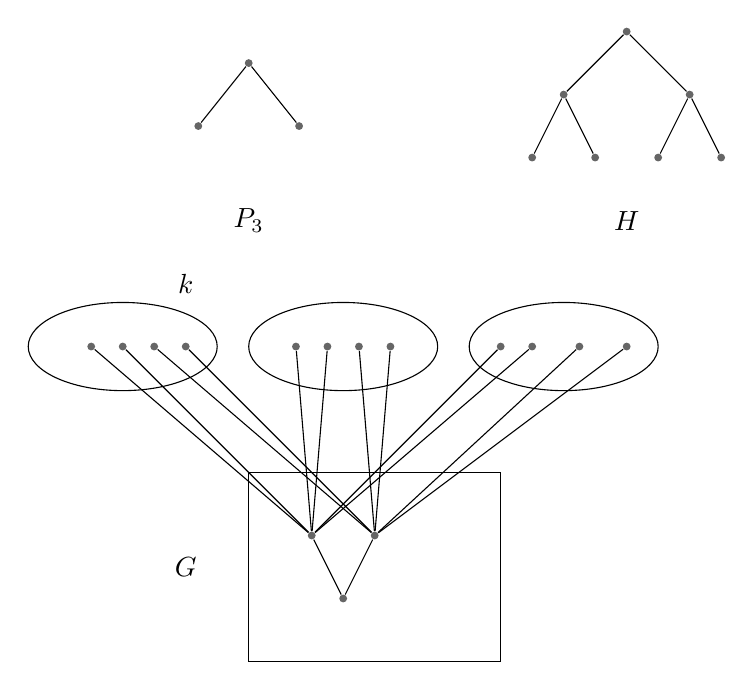
\begin{tikzpicture}
	 [scale=.8,auto=center,every node/.style={circle,fill=black!60,inner sep=1pt}]
	\node (n1) at (18,12) {};
	  \node (n2) at (17,11) {};
	  \node (n3) at (19,11) {};
	  \node (n4) at (16.5,10) {};
 	  \node (n5) at (17.5,10) {};
	  \node (n6) at (18.5,10) {};
   	  \node (n7) at (19.5,10) {};

   	  \node[fill=none] (L1) at (18,9) {$H$};

	\foreach \from/\to in {n1/n2,n1/n3,n2/n4,n2/n5,n3/n6,n3/n7}
    \draw (\from) -- (\to);

	  \node (a1) at (12,11.5) {};
	  \node (a2) at (11.2,10.5) {};
	  \node (a3) at (12.8,10.5) {};

	\foreach \from/\to in {a1/a2,a1/a3}
    \draw (\from) -- (\to);

   	  \node[fill=none] (L2) at (12,9) {$P_3$};

	    \draw (12,5) rectangle (16,2);

	  \node (B) at (13,4) {};
	  \node (C) at (14,4) {};
	  \node (A) at (13.5,3) {};

	\foreach \from/\to in {A/B,A/C}
    \draw (\from) -- (\to);

	\node[fill=none] (L3) at (11,3.5) {$G$};


    \draw (10,7) ellipse (1.5cm and 0.7cm);

     \node (r4) at (9.5,7) {};
 	  \node (r5) at (10,7) {};
	  \node (r6) at (10.5,7) {};
   	  \node (r7) at (11,7) {};


	\foreach \from/\to in {B/r4,B/r5,C/r6,C/r7}
    \draw (\from) -- (\to);


     \node (s4) at (12.75,7) {};
 	  \node (s5) at (13.25,7) {};
	  \node (s6) at (13.75,7) {};
   	  \node (s7) at (14.25,7) {};

	\foreach \from/\to in {B/s4,B/s5,C/s6,C/s7}
    \draw (\from) -- (\to);

     \node (t4) at (16,7) {};
 	  \node (t5) at (16.5,7) {};
	  \node (t6) at (17.25,7) {};
   	  \node (t7) at (18,7) {};


	\foreach \from/\to in {B/t4,B/t5,C/t6,C/t7}
    \draw (\from) -- (\to);


    \draw (13.5,7) ellipse (1.5cm and 0.7cm);
    \draw (17,7) ellipse (1.5cm and 0.7cm);

    \node[fill=none] (L4) at (11,8) {$k$};

\end{tikzpicture}
}



\end{document}
